\documentclass[12pt, twoside]{article}
\usepackage{jmlda}
\newcommand{\hdir}{.}

\usepackage{dsfont}

\usepackage{csvsimple}

\begin{document}

\title
    [Порождение признаков с помощью локально-аппроксимирующих моделей] % краткое название; не нужно, если полное название влезает в~колонтитул
    {Порождение признаков с помощью локально-аппроксимирующих моделей}
\author
    [Максим~Христолюбов, В.\,В.~Стрижов] % список авторов (не более трех) для колонтитула; не нужен, если основной список влезает в колонтитул
    {Максим~Христолюбов, В.\,В.~Стрижов, Александра~Гальцева, Данил~Сайранов} % основной список авторов, выводимый в оглавление
    [Максим~Христолюбов, В.\,В.~Стрижов, Александра~Гальцева, Данил~Сайранов] % список авторов, выводимый в заголовок; не нужен, если он не отличается от основного
\email
    {khristolyubov.me@phystech.edu}
\thanks
    {Работа выполнена при
     %частичной
     финансовой поддержке РФФИ, проекты \No\ \No 00-00-00000 и 00-00-00001.}
\organization
    {$^1$Московский физико-технический институт}
\abstract
    {В работе рассматривается классификация временных рядов акселерометра. Классификация производится методам порождения признаков с помощью локально аппроксимирующих моделей. Предполагается, что точки временного ряда можно разбить на кластеры, соответствующие разным классам. Предлагается выделить квазипериодические сегменты из временных интервалов точек, принадлежащих одному кластеру. В качестве признаков для классификации использовать параметры моделей, обученных на этих сегментах. Исследуется вопрос информативности порожденных признаков и возможность идентификации по ним владельца прибора или его физических параметров.
	
\bigskip
\noindent
\textbf{Ключевые слова}: \emph {временной ряд; классификация; кластеризация; сегментация временного ряда; локально аппроксимирующая модель}
}

\maketitle
\linenumbers

\section{Введение}

В статье изучается задача идентификации движений человека по временным рядам. В дополнении к этому исследуется возможность выделение атрибутивных паттернов, которые могут быть использованы для определения личности или физических параметров субъектов данных в дополнении к их деятельности. Классификация временных рядов находит широкое применение в сфере здравоохранения.

Временные ряды являются объектами сложной структуры, требующие предварительной обработки и представления их в удобном для классификации виде. Необходимо отобразить исходный временной ряд в некоторое пространство признаков. Например, в статье \cite{Ivkin15} временной ряд аппроксимируется моделью, а признаками являются ее параметры. В качестве аппроксимирующей модели берется модель авторегрегрессии, а так же собственные числа траекторной матрицы, в случае модели сингулярного спектра. В работе \cite{Karasikov16} проводится разбиение временных рядов на сегменты фиксированной длины, на которых впоследствии обучается локально-аппроксимирующая модель. Для аппроксимации используется линейная модель, модель авторегрессии и коэффициенты преобразования Фурье. В \cite{Anikeev18} предлагается более разумный способ сегментации, а так же применяется аппроксимации сплайнами. Еще более общий подход к способу сегментации посредством нахождения главных компонент траекторной матрицы, рассмотрен в \cite{Motrenko16}. В \cite{Bochkarev18} сравниваются между собой перечисленные выше подходы.

Метод кластеризации точек, соответствующих участкам разной деятельности, с помощью методы главных компонента (SSA, алгоритм гусеница \cite{Danilov97}) рассмотрен в \cite{Grabovoy20}. На участках, содержащих точки одного кластера, уже можно применять описанные выше методы. Другим подходом к классификации точек временного ряда на основе нейросетей рассмотрены в \cite{Dafne19} и \cite{Cinar18}.

В работе исследуется оптимальное признаковое описание точек пр которому можно будет идентифицировать род деятельности человека. Предлагается построить набор локально-аппроксимирующих моделей и выбрать наиболее адекватные. Производится построение пространства описаний элементарных движений. Новизна работы заключается в исследовании зависимости решений задач классификации действий и предсказания параметров человека.

\section{Постановка задачи}

Пусть имеется исходный временной ряд $\mathbf{d}=\{d_i\}_{i=1}^M\in \mathds{R}^M$. Предполагается, что он состоит из последовательности сегментов: 
\begin{equation}\label{eq0}
\mathbf{d}=[\mathbf{s}_1, \ldots \mathbf{s}_N],
\end{equation}
 где $\mathbf{s_i}\in Y$, $|Y|$~---~число различных действий (кластеров). Считается, что периоды $|\mathbf{s}|$ сегментов различаются незначительно, причем известен максимальный период $|\mathbf{s}|\leq T$.

Требуется решить задачу классификации точек ряда: $$R:\mathcal{I}\rightarrow Y,$$ где $\mathcal{I}=\{1,\ldots M\}$~---~моменты времени, на котором задан временной ряд, а $Y$~---~метки классов.

Каждый моменты времени $k$ отобразим с помощью $g:\mathcal{I}\rightarrow R^T$ в временной сегмент $\mathbf{x}_k$ длины $3T$, по предположению, содержащий всю информацию о локальном поведении ряда:
\begin{equation}\label{eq1}
h(k) = \mathbf{x}_k = \{d_i\}_{i=k-2T}^{k+T}.
\end{equation}

\begin{figure}[H]
\center{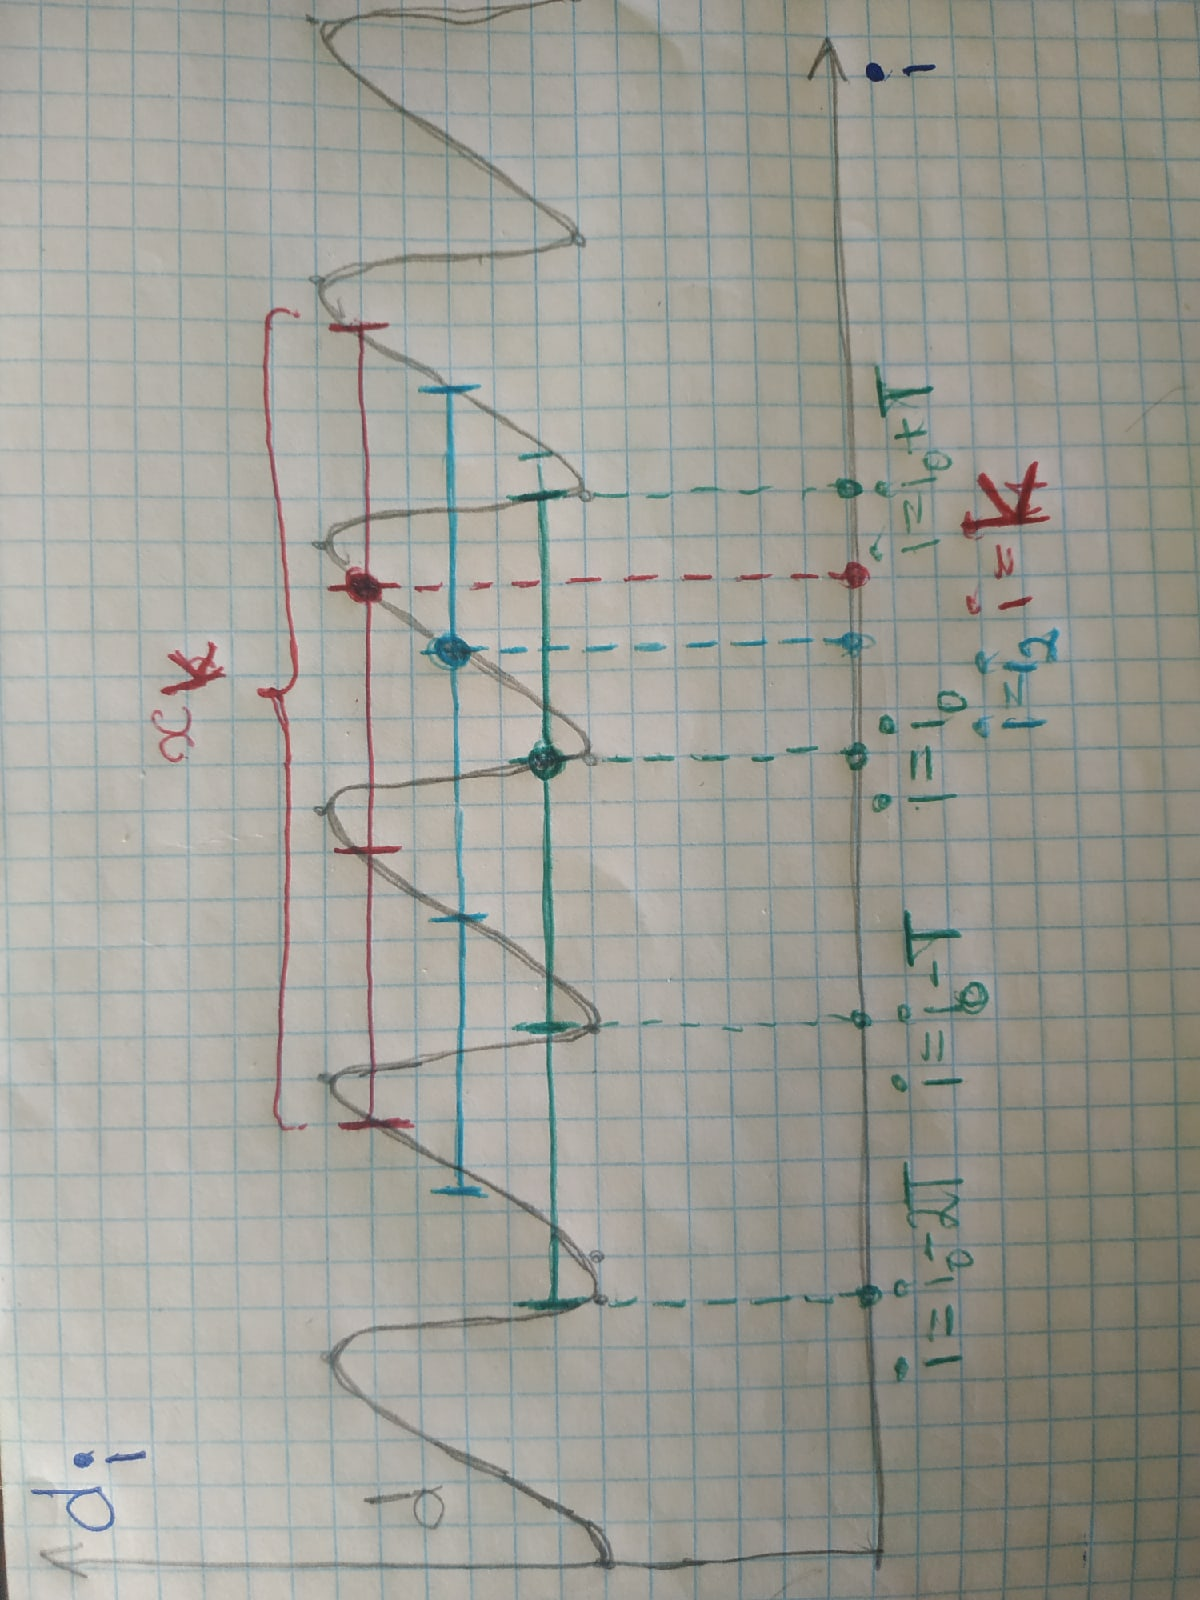
\includegraphics[scale=0.2, angle = -90]{prob}}
\caption{ Временной ряд}
\label{fig:image}
\end{figure}


Полученные сегменты $\mathbf{x} \in \mathcal{X}$~---~объекты сложной структуры, представленные временными рядами. Рассматривается задача классификации, а именно восстановление зависимости $$y=f(\mathbf{x}),$$ где $y\in Y$~---~пространство ответов. Тогда исходная задача классификации представляет собой $R=f\circ h$.

Заданы выборка объектов сложной структуры и ответов $\mathfrak{D}=\{(\mathbf{x}_i,y_i)\}_{i=1}^m$. Задача состоит в нахождении функции $f$, минимизирующие суммарные потери на выборке $\mathfrak{D}$, при заданной функция потерь $\mathscr{L}:(\mathcal{X},F,Y)\rightarrow R$, $\mathscr{L}(f(\mathbf{x}_i),y_i)$, характеризующая ошибку классификации функции $f\in F$ на элементе $\mathbf{x}_i$. 

Пусть $$w:\mathcal{X}\rightarrow W = \mathds{R}^n$$~---~процедура построения признакового описания сегмента. Тогда $W$~---~пространство признаков, в котором производится классификация временных рядов.

Пусть $b$~---~алгоритм многоклассовой классификации: 
\begin{equation}\label{classif}
b:W\rightarrow Y
\end{equation}

Тогда $f$ ищется в среди композиций вида 
$$f=b\circ w$$
Для любого $w$ можно найти оптимальное значение вектора $\hat\mu$ параметров классификатора $b(w(x),\mu)$, минимизирующего функционал качества: 
\begin{equation}\label{func_loss}
\hat\mu=\argmin_\mu \widetilde{Q}(b\circ w,\mathfrak{D})
\end{equation}

Оптимальный метод обучения для конкретного способа задания пространства признаков $w$ и выбранной модели классификации, определяется по скользящему контролю

$$\hat{f_{w}}=\argmin\limits_{w}\widehat{CV}(f_{w},\mathfrak{D}),$$ 
где $\widehat{CV}(f,\mathfrak{D})$~---~внешний контроль качества методы обучения $f$, $\mathfrak{D}=\mathfrak{L}\sqcup\mathfrak{E}$:
 \begin{equation}\label{CV}
\widehat{CV}(f, \mathfrak{D})=\frac{1}{r}\sum\limits_{k=1}^r Q(f^*(\mathfrak{L}),\mathfrak{E})
\end{equation}

В качестве функционала качества используется 
$$Q(f,\mathfrak{L})=\frac{1}{|\mathfrak{L}|}\sum\limits_{(\mathbf{x},y)\in\mathfrak{L}}|\{(\mathbf{x},y)\in\mathfrak{L}|f(\mathbf{x})=y\}|,$$ 
а в оценке точности классификации объектов класса $c\in Y$ используется модифицированный функционал качества 
$$Q_c(f,\mathfrak{L})=\frac{1}{|\mathfrak{L}|}\sum\limits_{(\mathbf{x},y)\in\mathfrak{L}}\frac{|\{(\mathbf{x},y)\in\mathfrak{L}|f(\mathbf{x})=y=c\}|}{|\{(\mathbf{x},y)\in\mathfrak{L}|y=c\}|}$$


\section{Порождение признаков}

Модель $g$, с помощью которой производится порождение признаков временных сегментов, называется локально-аппроксимирующей моделью, в силу локальности рассматриваемого сегмента \ref{eq1} временного ряда \ref{eq0}. В качестве признакового описания сегмента предлагается использовать вектор оптимальных параметров $w$ модели: 
$$\mathbf{w}(\mathbf{x})=\argmin\limits_{\mathbf{w}}||\hat{\mathbf{x}}(\mathbf{w},\mathbf{x})-\mathbf{x}||_2$$

Для порождения признакового описания $\hat{\mathbf{w}}$ для $L$-мерного временного ряда последовательно применяется операция порождения признаков к каждому одномерному ряду, и все полученные векторы признаков $\mathbf{w}_l$ объединяются:
$$\widetilde{\mathbf{w}} = \mathbf{w}_1\times \ldots \times \mathbf{w}_L,$$
где $\times$ это операция конкатенации, $\mathbf{w}\in W$, $\widetilde{\mathbf{w}} \in W^L$


\subsection{Авторегрессия}
Модель авторегрессии AR($2$T) предсказывает следующее значение сегмента (\ref{eq1}) как линейную комбинацию $2T$ предыдущих:
$$\hat{x}^{(k)}=w_0+\sum\limits_{j=1}^{2T} w_i x^{(k-j)}.$$

Для нахождения оптимального вектора параметров $\mathbf{w}$ решается задача минимизации:
$$\mathbf{w}(\mathbf{x})=\argmin_{\mathbf{w}}(||\mathbf{x}-\hat{\mathbf{x}}||_2^2=\argmin_{\mathbf{w}}||\mathbf{x}-\mathbf{X}\mathbf{w}||_2^2=(\mathbf{X}^\mathsf{T}\mathbf{X})^{-1}\mathbf{X}^\mathsf{T}\mathbf{x},$$
где $\mathbf{X}$~---~матрица Ганкеля:

\begin{equation*}\label{gankel}
\mathbf{X} = \left(
\begin{array}{cccc}
x^{(1)} & x^{(2)} & \ldots & x^{(T)}\\
x^{(2)} & x^{(3)} & \ldots & x^{(T+1)}\\
\vdots & \vdots & \ddots & \vdots\\
x^{(2T+1)} & x^{(2T+2)} & \ldots & x^{(3T)}
\end{array}
\right).
\end{equation*}

\subsection{ Анализ сингулярного спектра}
Рассмотрим модель SSA порождения данных. Поставим в соответствие временному сегменту $\mathbf{x}$ его траекторную матрицу $\mathbf{X}$ \ref{gankel}. Ее сингулярное разложение 
$$\mathbf{X}^\mathsf{T}\mathbf{X}=\mathbf{V}\mathbf{H}\mathbf{V}^\mathsf{T},\quad \mathbf{H} = \text{diag}(h_1,\ldots h_T).$$ 
$h_1\ldots h_T$~---~собственные числа матрицы $\mathbf{X}^\mathsf{T}\mathbf{X}$. Первые десять собственных чисел берется в качестве нового признакового описания $\mathbf{w}=[h_1,\ldots h_{10}]$.  

\subsection{ Дискретное преобразование Фурье}
К временному сегменту применяется дискретное преобразование Фурье:
$$w_k = \sum\limits_{n=1}^{T}x^{(k)}e^{-\frac{2\pi i}{T}kn},$$
или же в матричном виде $\mathbf{w} = \mathbf{Z}x,$ где матрица $\mathbf{Z}$:

\begin{equation*}
\mathbf{Z} = \left(
\begin{array}{cccc}
e^{-\frac{2\pi i}{T}} & e^{-\frac{2\pi i}{T}\cdot 2} & \ldots & e^{-\frac{2\pi i}{T}\cdot T}\\
e^{-\frac{2\pi i}{T}\cdot 2}\ & e^{-\frac{2\pi i}{T}\cdot 4}\ & \ldots & e^{-\frac{2\pi i}{T}\cdot 2\cdot T}\\\
\vdots & \vdots & \ddots & \vdots\\
e^{-\frac{2\pi i}{T}\cdot 3T}\ & e^{-\frac{2\pi i}{T}\cdot 3T\cdot 2}\ & \vdots & e^{-\frac{2\pi i}{T}\cdot 3T\cdot T}\
\end{array}
\right).
\end{equation*}

В качестве признаков $\mathbf{w}$ берутся $T$ коэффициентов Фурье.


\section{Вычислительный эксперимент}

В качестве вычислительного эксперимента решаются две задачи:  классификация типов активности человека и классификация пола человека. 

Условия измерения данных: данные~---~это измерения акселерометра и гироскопа, встроенных в мобильное устройство IPhone 6s, хранящегося в переднем кармане брюк участника. Временные ряды содержат значения ускорения человека и углы ориентацию телефона для каждой из трёх осей~---~всего шесть временных рядов. Частота дискретизации составляет $50$ Гц. Метками классов служат: подъем по лестнице вверх, спуск по лестнице вниз, ходьба, бег трусцой, сидение, лежание. Данные собраны с $24$ участников, для каждого из  которых известны рост, вес, возраст и пол. Данные собирались в условиях проведения эксперимента: участникам выдавали телефон и просили выполнять одно из шести действий в течении двух минут \url{https://github.com/mmalekzadeh/motion-sense}.

Для эксперимента берется шесть временных рядов в $39000$ временных моментов ($780$ секунд). Данные снимаются с четырех человек (двое мужчин и две женщины), которые выполняют подъем или спуск по лестнице (два типа деятельности).

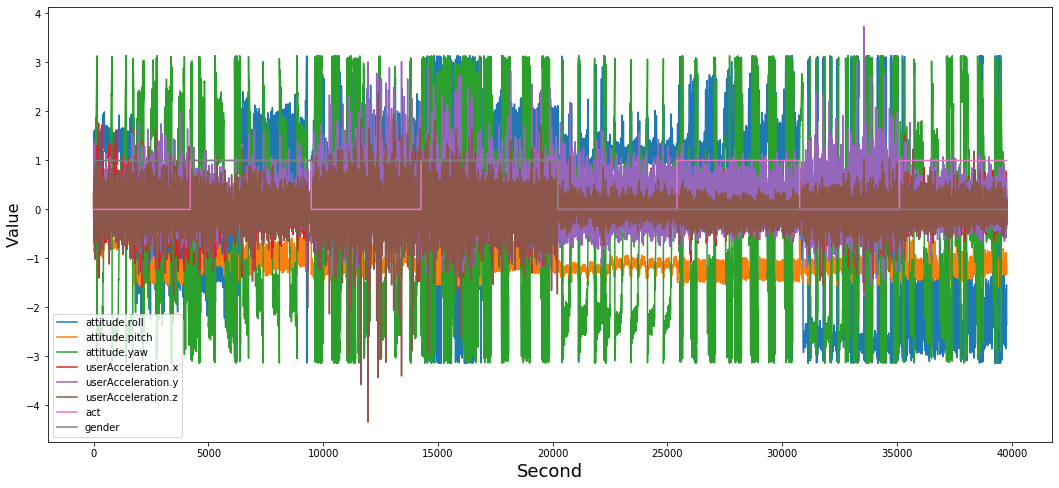
\includegraphics[scale=0.43]{data}

Производится классификация не всех моментов времени, а только каждый десятый момент времени (пять в секунду), а класс остальных моментов времени определяется классом ближайшего классифицированного момента времени.. Это позволяет уменьшить размер выборки для классификации с $39000$ точек до $3900$, если классифицировать каждую десятую точку.

На соответствующих моментам времени сегментах строятся локально-аппроксимирующие модели, чьи параметры используются в качестве признаков. Сравниваются информативность признаков, порожденных моделью авторегресси (с $50$ членами), коэффициенты ряда Фурье ($100$ для каждого ряда), $10$ сингулярных числа SSA разложения. 

Отбор оптимальных признаков производится методом Sequential Backward Floating Selection \cite{Somol10} для выбранной модели классификации. 

Для классификации используются две модели $b$ (\ref{classif}).

1) Логистическая регрессия \cite{Peng02} c $l_2$ регуляризацией, для которой $\widetilde{Q}$ в (\ref{func_loss}) задается выражением:
$$\widetilde{Q}(w,\mathfrak{D}) = \frac{1}{2}w^Tw + \sum\limits_{i=1}^{|\mathfrak{D}|} \ln(1+exp(-y_i(X_i^Tw+c))).$$

2) C-Support Vector Classification \cite{Liu11}, минимизирующий функцию: 
\begin{align}\begin{aligned}\min_ {w, b, \zeta} \frac{1}{2} w^T w + C \sum_{i=1}^{n} \zeta_i,\\\begin{split}\textrm {subject to } & y_i (w^T \phi (x_i) + b) \geq 1 - \zeta_i,\\
& \zeta_i \geq 0, i=1, ..., n,\end{split}\end{aligned}\end{align}
где $K(x_i, x_j) = \phi (x_i)^T \phi (x_j)$~---~ядро.

Отдельно решаются задачи классификации активности и пола человека. После этого для проверки наличия причинно-следственной зависимости между активностью и полом производится обучения на расширенной матрице признаков: сначала решается одна задача классификации, а потом полученный вектор решения используется как признак для решения второй задачи.

\begin{table}[H]
\caption{Среднее и дисперсия верных классификаций при кросс-валидации}
\begin{table}[H]
\begin{tabular}{|l|l|l|l|l|l|l|l|l|}
\hline
               & mean(activity)   & std(activity) & mean(gender) & std(gender) & Сommon features\\ \hline
Log Regression & 0.888 & 0.162 & 0.928  & 0.212    & 0 \\
after adding   & 0.882 & 0.170 & 0.955  & 0.112    &     \\ \hline
SVC            & 0.911 & 0.143 & 0.962  & 0.110    & 0 \\
after adding   & 0.883 & 0.191 & 0.960  & 0.087    & \\ \hline
\end{tabular}
\end{table}

\end{table}

Результаты показывают, что использование пола при определении типа деятетльности не улучшает точности модели, а использование типа актиности при определении пола значительно уменьшает ошибки и увеличивает устойчивость модели логистической регрессии. Ошибки модели C-Support Vector Classification не уменьшаются, но увеличивается устойчивость.

\begin{figure}[H]
\center{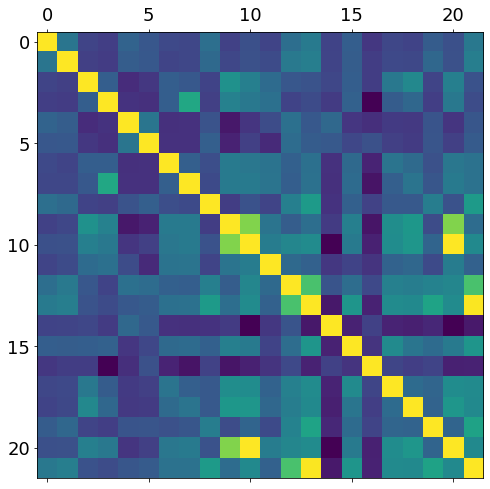
\includegraphics[scale=0.4]{corr}}
\caption{ Корреляционная матрица оптимальных признаков}
\label{fig:image}
\end{figure}

Первые $13$ признаков~---~это оптимальные признаки для решения задачи классификации активности, последние $7$ признаков~---~оптимальные в задаче классификации пола.


\section{ Дополнение}
\label{dop}

Алгоритм отбора Sequential Backward Floating Selection состоит из двух шагов:

1) Выбор признака $w^- = \argmax\limits_{w^- \in w} \max\limits_{f}\widehat{CV}(f, \mathfrak{D}(w^k-w^-)$, без которого модель классификации, полученная на оставшихся признаках дает максимальное значение $\widehat{CV}(f^*, \mathfrak{D}(w^k-w^-)$, где $\widehat{\hat{CV}}$ это (\ref{CV}), и отбрасывание $w^-$ из вектора признаков $w^{k-1}=w^k-w^-$.

2) Если существует признак $w^+$, добавив который, можно получить большее значение функции, чем она была на выборке c признакми, которые были до предыдущего шага $\max\limits_f \widehat{CV}(f, \mathfrak{D}(w^{k-1}+w^-))<\max\limits_f \widehat{CV}(f, \mathfrak{D}(w^{k-1}+w^+))$, то добавить этот признак к вектору признаков $w^k = w^{k-1}+w^+$.

Эти шаги повторяются, пока не останется $K$ оптимальных признаков, то есть пока не будет достигнуто равенство $k=K$.

\maketitleSecondary
\English
\begin{thebibliography}{99}

\bibitem{Ivkin15}
	\BibAuthor{N.~P.~Ivkin, M.~P.~Kuznetsov.}. 2015.
	 Time series classification algorithm using combined feature description. .
	\BibJournal{Machine Learning and Data Analysis} (11):1471–1483.

\bibitem{Karasikov16}
	\BibAuthor{V.~V.~Strijov, M.~E.~Karasikov.} 2016.
	Feature-based time-series classification
	\BibJournal{Informatics}
	\BibDoi{10.3114/S187007708007}.
	
\bibitem{Anikeev18}	
	\BibAuthor{D.A. Anikeev, G.O. Penkin, V.V. Strijov}. 2018.
	Local approximation models for human physical activity classification~//
	\BibJournal{Informatics}
	\BibDoi{10.14357/19922264190106}.

\bibitem{Isachenko16}
	\BibAuthor{V.V. Strijov, R.V. Isachenko.}. 2016.
	 Metric learning in multiclass time series classification problem.
	\BibJournal{Informatics and Applications} (10(2)):48–57.

\bibitem{Popova16}
	\BibAuthor{V.V. Strijov, Andrew~Zadayanchuk, Maria~Popova.}. 2016.
	 Selection of optimal physical activity classification model using measurements of accelerometer.
	\BibJournal{Information Technologies}  (22(4)):313–318.

\bibitem{Motrenko16}
	\BibAuthor{Strijov~V.V., Motrenko~A.P.}. 2016.
	 Extracting fundamental periods to segment human motion time series.
	\BibJournal{Journal of Biomedical and Health Informatics}  20(6):1466 – 1476.

\bibitem{Ignatov15}
	\BibAuthor{Strijov~V.V., Ignatov A.}. 2015.
	 Human activity recognition using quasiperiodic time series collected from a single triaxial accelerometer.
	\BibJournal{Multimedia Tools and Applications}  pages 1–14.
	
\bibitem{Bochkarev18}
	\BibAuthor{Isachenko R.V., Bochkarev А.М., Zharikov I.N., Strijov V.V.}. 2018.
	Feature Generation for Physical Activity Classification.
	\BibJournal{Artificial Intelligence and Decision Making}  3 : 20-27.

\bibitem{Dafne19}
	\BibAuthor{Dafne van Kuppevelt, Joe Heywood, Mark Hamer, Séverine Sabia, Emla Fitzsimons, Vincent van Hees}. 2019.
	 Segmenting accelerometer data from daily life with unsupervised machine learning.
	\BibJournal{PLOS ONE}
    \BibDoi{10.5255/UKDA-SN-8156-3}.
    
\bibitem{Sabatini10}
    \BibAuthor{Andrea Mannini, Angelo Maria Sabatini}. 2010.
    Machine Learning Methods for Classifying Human Physical Activity from On-Body Accelerometers
    \BibJournal{PubMed}
    \BibDoi{10.3390/s100201154}.
    
\bibitem{Grabovoy20}
	\BibAuthor{Grabovoy A.V., Strijov V.V}. 2020.
	Quasiperiodic time series clustering for human activity recognition
	\BibJournal{Lobachevskii Journal of Mathematics}
	
\bibitem{Danilov97}
	\BibAuthor{D.L. Danilov and A.A. Zhiglovsky}. 1997.
	\BibTitle{Main components of time series: method "Gesenitsa" (St. Petersburg)}
	
\bibitem{Cinar18}
	\BibAuthor{ Y.G. Cinar and H. Mirisaee}. 2018.
	Period-aware content attention RNNs for time series forecasting with missing values
	\BibJournal{”Neurocomputing}  312, 177–186
    
\bibitem{Malekzadeh19}
	\BibAuthor{Malekzadeh, Mohammad and Clegg, Richard G. and Cavallaro, Andrea and Haddadi, Hamed}. 2019.
	\BibTitle{Mobile Sensor Data Anonymization}  pages 49--58.
    \Bibbooktitle{Proceedings of the International Conference on Internet of Things Design and Implementation}
    \BibDoi{10.1145/3302505.3310068}.
    
\bibitem{Somol10}
	\BibAuthor{Petr Somol, Jana, Novovicova, Pavel Pudil}. 2010.
	Efficient Feature Subset Selection and Subset Size Optimization
    \BibDoi{10.5772/9356}.
    
\bibitem{Peng02}
	\BibAuthor{Joanne Peng, Kuk Lida Lee, Gary M. Ingersoll}. 2002.
	An Introduction to Logistic Regression Analysis and Reporting
    \BibDoi{10.1080/00220670209598786}.
    
\bibitem{Liu11}
	\BibAuthor{Quanzhong Liu, Chihau Chen, Yang Zhang, Zhengguo Hu}. 2011.
	Feature selection for support vector machines with RBF kernel
    \BibDoi{10.1007/s10462-011-9205-2}.
 

\printbibliography
  	     	
\end{thebibliography}


\end{document}
